Una de las primeras características que cabe resaltar de golang es que no tiene clases ni herencia. como estructura
principal de datos tiene los structs. Si queremos que las instancias se creen bajo una misma logica que no se pueda saltar
debemos definir una interfaz y crear un struct que la implemente. los struct pueden implementar metodos pasandose a si mismos por referencia en una funcion

\begin{lstlisting}[label={lst:lstlisting}]

package ClassEquivalentExample

type Class interface {
	Get() string
	Set(newValue string)
}

type class struct {
	variable string
}

func NewClass() Class {
	return &class{"default"}
}

func (class *class) Get() string {
	return class.variable
}

func (class *class) Set(newValue string) {
	class.variable = newValue
}

\end{lstlisting}

lo cual resulta en un diagrama UML

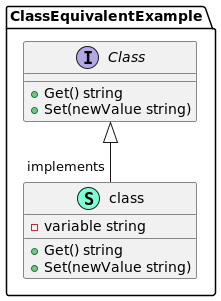
\includegraphics{./part/Proyecto_ejecutivo/memoria_constructiva/ClassEquivalentInGolang}

por qué es importante concebir esta estructura:

\begin{itemize}
    \item Evitamos la instanciación no consistente, lo cual solo se garantiza a traves del método si exportado NewClass
    \item evitamos accesos no deseados al seteo de variables. Si las pusieramos publicas seria posible.
\end{itemize}

como contrapartida tenemos que escribir más codigo. poniendo como comparación una clase java o C++ no podemos decir que en cantidad de lineas escritas se aumente o disminuya. En cuestión de conceptos aprendidos en Golang sólamente trabaja con interfaces y structs contra el concepto de clase y herencia.

